\section{OpenETCS case study}

\todo{This section is intentionnally empty for the moment : }

\todo{it will be completed when the document provided by Alstom on API  will be available.}

\begin{comment}
From QA :

The EVC (European Vital Computer) is the heart of the ERTMS onboard system. This safety
computer implements the functions of the SRS subset 026 of UNISIG (for SRS versions beginning
with baseline 3, published by ERA) in order to guarantee the safety of the train movements.
The OpenETCS scope of application is related to the only EVC part of whole ERTMS system.
The Track-side part of the ETCS (the Radio Based Control) is excluded from the project activities,
and only considered through its interfaces with the On-Board part of ETCS.

\end{comment}

\subsection{Aim of the OpenETCS project}

\begin{comment} 
The goal of The OpenETCS project is to provide a formal model of the On board Unit from the Subset 26 specification.

The following sections are going to give a high level description of this case study and expected elements.

Detailled specification of the system will be given during WP3 activities.
\end{comment}


\subsection{High level description of the  case study}
high level description of the subset + link to reference documentation (subset 26)


\req{The model shall comply all OBU ETCS mandatory requirements for level upto 2, in the 
functional perimeter provided by the Functional Architecture.}
\subreq{The model shall comply the OBU part of SUBSET-26-3.3.0.}



\subreq{The reference ETCS baseline shall be modified only by project decision, according
to the QA Plan.}
\subreq{All divergences against the chosen baseline shall be documented and tracked, according
to the QA Plan.}

\subsection{Environement and abstract architecture}
high level description of the environement  of the system  and main function

\begin{figure}[h]
  \centering
  \fbox{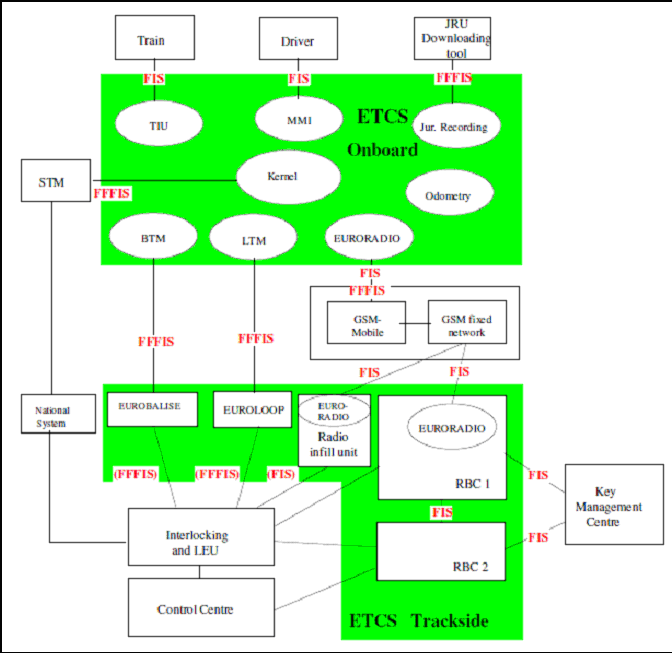
\includegraphics[width=4in]{archi}}
  \caption{Architecture}
  \label{fig:architecture}
\end{figure}

\tbc

\subsection{Safety properties}
reference document subset 091 to the list of safety properties


\tbc
